%!TEX root = ../surface_reconstruction.tex


\section{Описание последовательного алгоритма}

Пусть точки $p_i \in R^{3}, i \in \{1, . . . , N\}$, взяты с
поверхности S (возможно, с шумом измерения). Цель состоит в том, чтобы спроецировать точку $r \in R^{3}$ вблизи S на двумерную поверхность SP, аппроксимирующую $p_i$. Процедура MLS мотивирована дифференциальной геометрией, а именно тем, что поверхность может быть локально аппроксимирована функцией.

Эталонная плоскость: 
 Локальная плоскость $ H = \{x \mid \langle n, x \rangle - D = 0, x  \in R^{3}\}, n \in R^{3},  \parallel n \parallel = 1 $ вычисляется так, чтобы минимизировать локальную взвешенную сумму квадратов расстояний точек pi до плоскости (см. рис. \ref{fig:0}). Веса, прикрепленные к $p_i$, определяются как функция расстояния от $p_i$ до проекции r на плоскость H, а не от расстояния до r. Предположим, что q является проекцией r на H, тогда H находится путем локальной минимизации
 \begin{equation}
     \sum_{i = 1}^{N}(\langle n, p_i \rangle - D)^{2} \theta(\parallel p_i - q \parallel)
     \label{eq:ref1}
 \end{equation}

где $\theta$ — гладкая монотонно убывающая функция, положительная на всем пространстве. Полагая $q = r + tn$ для некоторого $t \in R$, уравнение \ref{eq:ref1} можно переписать как: 
 $$\sum_{i = 1}^{N}(\langle n, p_i - r - tn \rangle)^{2} \theta(\parallel p_i - r - tn \parallel)$$
 
  Оператор $Q(r) = q = r + tn$ определяется как локальный минимум уравнения  с наименьшим t и локальной касательной плоскостью H вблизи r соответственно. Затем локальная эталонная область задается ортонормированной системой координат на H, так что q является началом этой системы.

\begin{figure}[h]
    \centering
    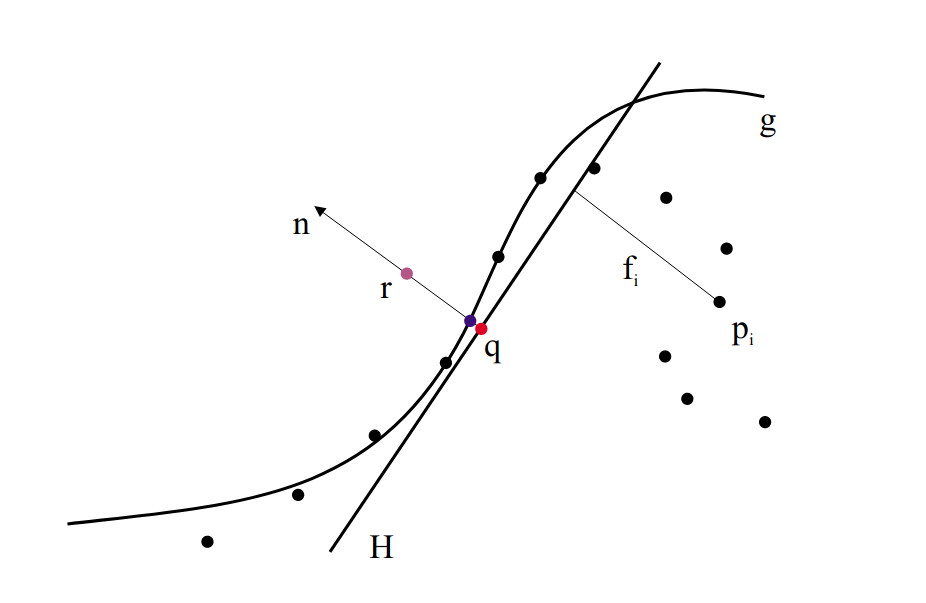
\includegraphics[scale=0.5]{images/0.png}
    \caption{Процедура проекции MLS: сначала создается локальная эталонная плоскость H для точки $p_j$. Проекция $p_j$ на H определяет начало координат q. Затем вычисляется локальная полиномиальная аппроксимация g высот $f_j$ точек $p_j$ над H. В обоих случаях вес для каждого из $p_j$ является функцией расстояния до q. Проекция $p_j$ на g является результатом работы алгоритма.}
    \label{fig:0}
\end{figure}


\section{Существующие алгоритмы}
\subsection{Оператор локально-оптимальной проекции(LOP)}
Происхождением метода является алгоритм Вайсфельда для решения задачи Ферма-Вебера о расположении точек, также известный как многомерная медиана L1. Это статистический инструмент, который традиционно применяется во всем мире для многомерных непараметрических точечных выборок, чтобы получить хорошего представителя для большого количества выборок при наличии шума и выбросов. Проблема была впервые известна как проблема оптимального местоположения Вебера ~\cite{WEBER}. Задача состояла в том, чтобы найти оптимальное место для промплощадки, минимизирующее стоимость доступа. В статистике проблема известна как медиана L1 ~\cite{BROWN, SMALL}.

Задача Ферма-Вебера (глобальная) о расположении точек рассматривается как пространственная медиана, поскольку, будучи ограничена одномерным случаем, она совпадает с одномерной медианой и наследует некоторые ее свойства в многомерной постановке.

Реконструкция с помощью оператора проекции имеет важное достоинство: она определяет непротиворечивую геометрию на основе точек данных и предоставляет конструктивные средства для повышения ее дискретизации. 
Оператор локально-оптимальной проекции без параметризации использует более примитивный механизм проецирования, но поскольку он не основан на локальной 2D-параметризации, он более надежен и хорошо работает в сложных сценариях. Кроме того, если точки данных взяты локально с гладкой поверхности, оператор обеспечивает аппроксимацию второго порядка, что приводит к правдоподобной аппроксимации выбранной поверхности.

Оператор LOP имеет две непосредственные функции: во-первых, его можно использовать в качестве этапа предварительной обработки для любого другого метода реконструкции более высокого порядка (например, RBF). LOP можно применять к необработанным отсканированным данным для создания чистого набора данных, в качестве средства эффективного уменьшения шума и выбросов, а также для упрощения определения ориентации и топологии локальной поверхности. Во-вторых, его можно использовать для уточнения данного набора данных.

Для множества точек данных $P = \{p_j\}_{j\in J} \subset \mathbf R^{3}$, LOP проецирует произвольное множество точек $X^{(0)} = \{x_i^{(0)} \} _{i \in I} \subset \mathbf R^{3}$ на множество $P$, где $I$, $J$ обозначают наборы индексов. Множество спроецированных точек $Q = \{q_i\}_{i\in I}$ определяется так, чтобы оно минимизировало сумму взвешенных расстояний до точек P относительно радиальных весов с центром в том же множестве точек Q. Кроме того, точки Q не должны быть слишком близко друг к другу. Эта структура индуцирует определение искомых точек Q как решение уравнения с фиксированной точкой 
$$Q = G(Q),$$
где
$$G(C) = argmin_{X = \{x_i\}_{i \in I}} \{E_1(X,P,C) + E_2(X,C)\},$$
$$E_1(X,P,C) = \sum_{i \in I} \sum_{j \in J}\parallel x_i - p_j \parallel \theta(\parallel c_i - p_j \parallel), $$ 
$$E_2(X, C) = \sum _{i^{'} \in I} \lambda_{i^{'}}\sum_{i \in I \setminus\{i^{'}\}} \eta(\parallel x_{i^{'}}- c_i  \parallel)\theta(\parallel c_{i^{'}} - c_i \parallel)$$

Здесь $\theta(r)$ — быстро убывающая гладкая весовая функция с компактным опорным радиусом $h$, определяющая размер радиуса влияния, $\eta(r)$ — другая убывающая функция, штрафующая $x_{i^{'}}$ за то, что они подходят слишком близко к другим точкам, и $\{\lambda_i\}_{i \in I}$ являются уравновешивающими членами, которые обозначены через $\mathbf \land$. В двух словах, термин $E_1$ заставляет спроецированные точки $Q$ аппроксимировать геометрию $P$, а член $E_2$ стремится  сохранить справедливое распределение точек $Q$. Правильные значения $\mathbf\land$ могут гарантировать степень аппроксимации второго порядка оператора LOP при условии, что данные отбираются с поверхности $C^{2}$.

\subsection{Радиальные базисные функции(RBFs)}
Радиальные базисные функции - это хорошо известный метод интерполяции разбросанных данных. Учитывая набор точек с заданными значениями функций, RBFs воспроизводят функции, содержащие высокую степень гладкости, посредством линейной комбинации радиально-симметричных базисных функций. Для реконструкции поверхности метод ~\cite{CARR} строит поверхность, находя скалярное поле со знаком, определенное через RBFs, набор нулевых уровней которого представляет поверхность. В частности, они используют глобально поддерживаемые базисные функции $\phi : R^{+} \rightarrow R$. Затем неявная функция $\Phi$ может быть выражена как:
$$\Phi(\mathbf{x}) = g(\mathbf{x}) + \sum_j\lambda_j\phi(\parallel \mathbf{x} - \mathbf{q_j} \parallel), $$
где $g(x)$ обозначает (глобально поддерживаемый) полином низкой степени, а базисные функции сосредоточены в узлах $\mathbf{q_j} \in R^{3} $. Неизвестные коэффициенты $λ_j$ находятся путем задания интерполяционных ограничений значения функции $\theta$ при $\mathbf{p_i} \in P;$ см. рис. \ref{fig:4}. Ограничения вне поверхности необходимы, чтобы избежать тривиального решения $f (\mathbf{x}) = 0$ для $\mathbf{x} \in R^{3}$. Положительные (соответственно отрицательные) ограничения устанавливаются для точек, смещенных в точке $\mathbf{p_i}$ по $\mathbf{n_i}$ в положительном (соответственно отрицательном) направлении. Интерполяция выполняется путем объединения точек ограничения на поверхности и вне поверхности как множество центров узлов $\mathbf{q_{j}} $. Коэффициенты $\mathbf{λ_i}$ находятся с помощью плотной линейной системы с n неизвестными, эффективно вычисляемой с помощью быстрых мультипольных методов ~\cite{CARR}. Преимущество использования глобально поддерживаемых базисных функций для реконструкции поверхности заключается в том, что результирующая неявная функция является глобально гладкой. Следовательно, RBFs могут быть эффективными для создания водонепроницаемой поверхности при наличии неравномерной выборки и недостающих данных. Однако, когда входные данные содержат умеренный шум, определение правильного размещения точек вне поверхности может стать сложной задачей (см. рис. \ref{fig:4} справа). 

\begin{figure}[h]
    \centering
    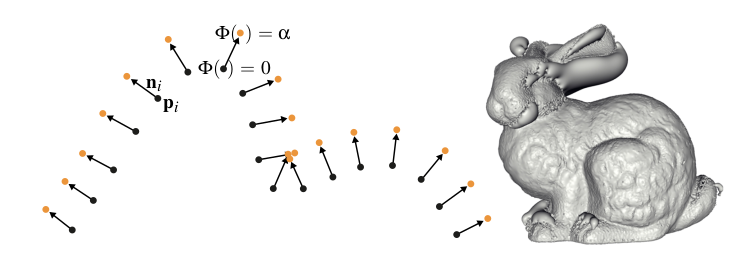
\includegraphics[scale=0.5]{images/4.png}
    \caption{(слева) Для RBFs оптимизируемое скалярное поле должно оцениваться как нуль в точках выборки $\Phi(\mathbf{p_i}) = 0$, в то время как при ограничениях вне поверхности $\Phi(\mathbf{p_i} + \alpha\mathbf{n_i}) = \alpha;$ этот выбор уместен, поскольку функции расстояния со знаком почти везде имеют норму единичного градиента. Кластер выборок вне поверхности показывает, насколько тщательно нужно задавать ограничения в областях с большой кривизной. (справа) Поверхность, реконструированная с помощью RBFs, обычно имеет серьезные геометрические и топологические артефакты, когда предоставляются противоречивые внешние ограничения.}
    \label{fig:4}
\end{figure}

\section{Параллелизм}

Процедура определения поверхности методом наименьших квадратов была представлена Левином ~\cite{LEVIN}. Параллельный вариант, модифицированного алгоритма MLS с использованием MPI, описан в алгоритме 1. Алгоритм предполагает что облако точек равномерно распределено по всем процессам. Поэтому часть P, доступная локально в процессе u, обозначается через $P^{(u)}$. Через $P_l^{u}$, $P_r^{u}$ обозначены левая и правая граница частей облака точек. Они последовательно получаются от соседних процессов обменами по топологии кольцо. Дополнительных коммуникаций не требуется, а остальные вычисления выполняются локально. В цикле по локальному облаку точек $P^{(u)}$ выполняется процедура проецирования MLS: сначала создается локальная эталонная плоскость H для точки $p_j$. Проекция $p_j$ на H определяет начало координат q. Затем вычисляется локальная полиномиальная аппроксимация g высот $f_j$ точек $p_j$ над H. В обоих случаях вес для каждого из $p_j$ является функцией расстояния до q. Проекция $p_j$ на g является результатом процедуры проецирования MLS. \\*
\textbf{Algorithm 1}  Parallel moving least squares with MPI \\*
\textbf{Input:} a data set of points $P = \{p_i\}$ $i = 1..n$ \\*
\textbf{Output:} a smooth surface SP (MLS surface) based on the input
points \\*
1: \textbf{for each} process u \textbf{do} \\*
2: \quad $P^{(u)} = read(P)$ // each process reads its part of point cloud $P^{(u)} = \{p_j\}$ $j = 1..m$ \\*
3: \quad $P\_l^{(u)} = send\_recv(P\_r^{(u-1)})$ // getting the left border\\* 
4: \quad $P\_r^{(u)} = send\_recv(P\_l^{(u+1)})$ // getting the right border\\*
5: \quad\textbf{for each} point $j = 1..m $ \textbf{do}\\*
6: \quad\quad$H = generate\_plane(p_j)$ \\*
7: \quad\quad$g = generate\_local\_polynomial\_approximation(H)$ \\*
8: \quad\quad$result\_point = project\_on\_polynom(p_j, polynom)$ \\*
9: \quad\textbf{end for} \\*




Параллельный алгоритм

\begin{figure}[h]
    \centering
    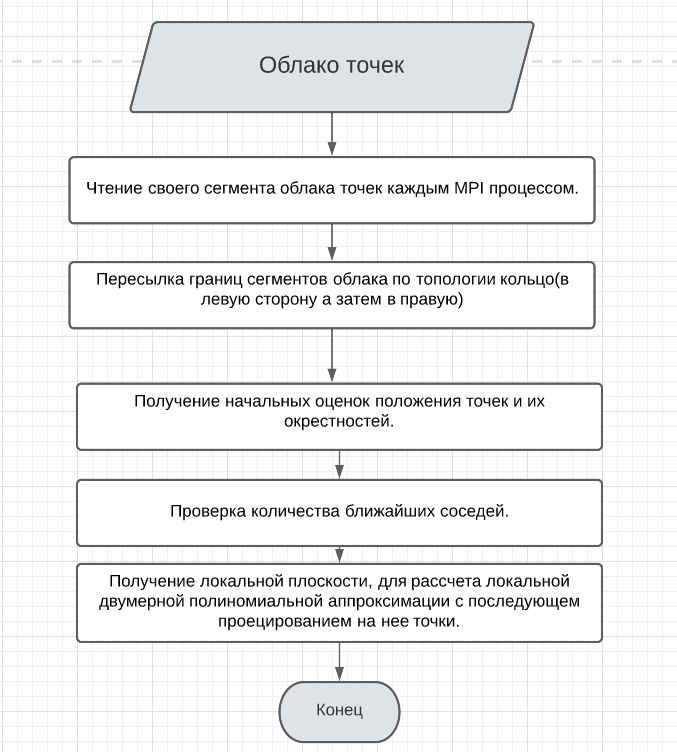
\includegraphics[scale=0.5]{1.png}
    \caption{Блок схема параллельной реализации алгоритма}
    \label{fig:mesh1}
\end{figure}


\begin{figure}
  \centering
  \subbottom[$np = 1$]{%
    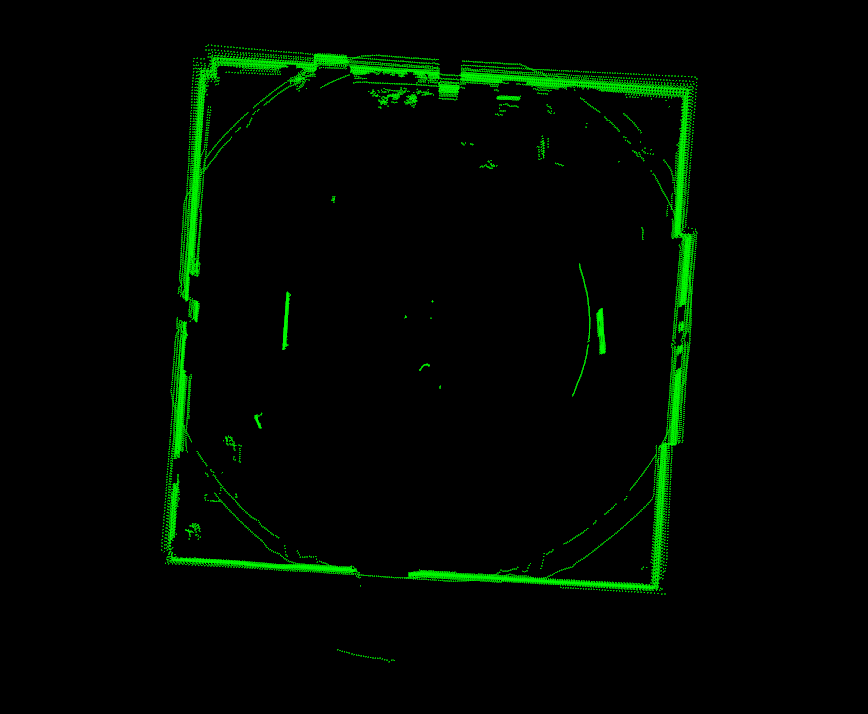
\includegraphics[width=0.4\linewidth]{images/3.png}}
  \subbottom[$np = 4$]{%
    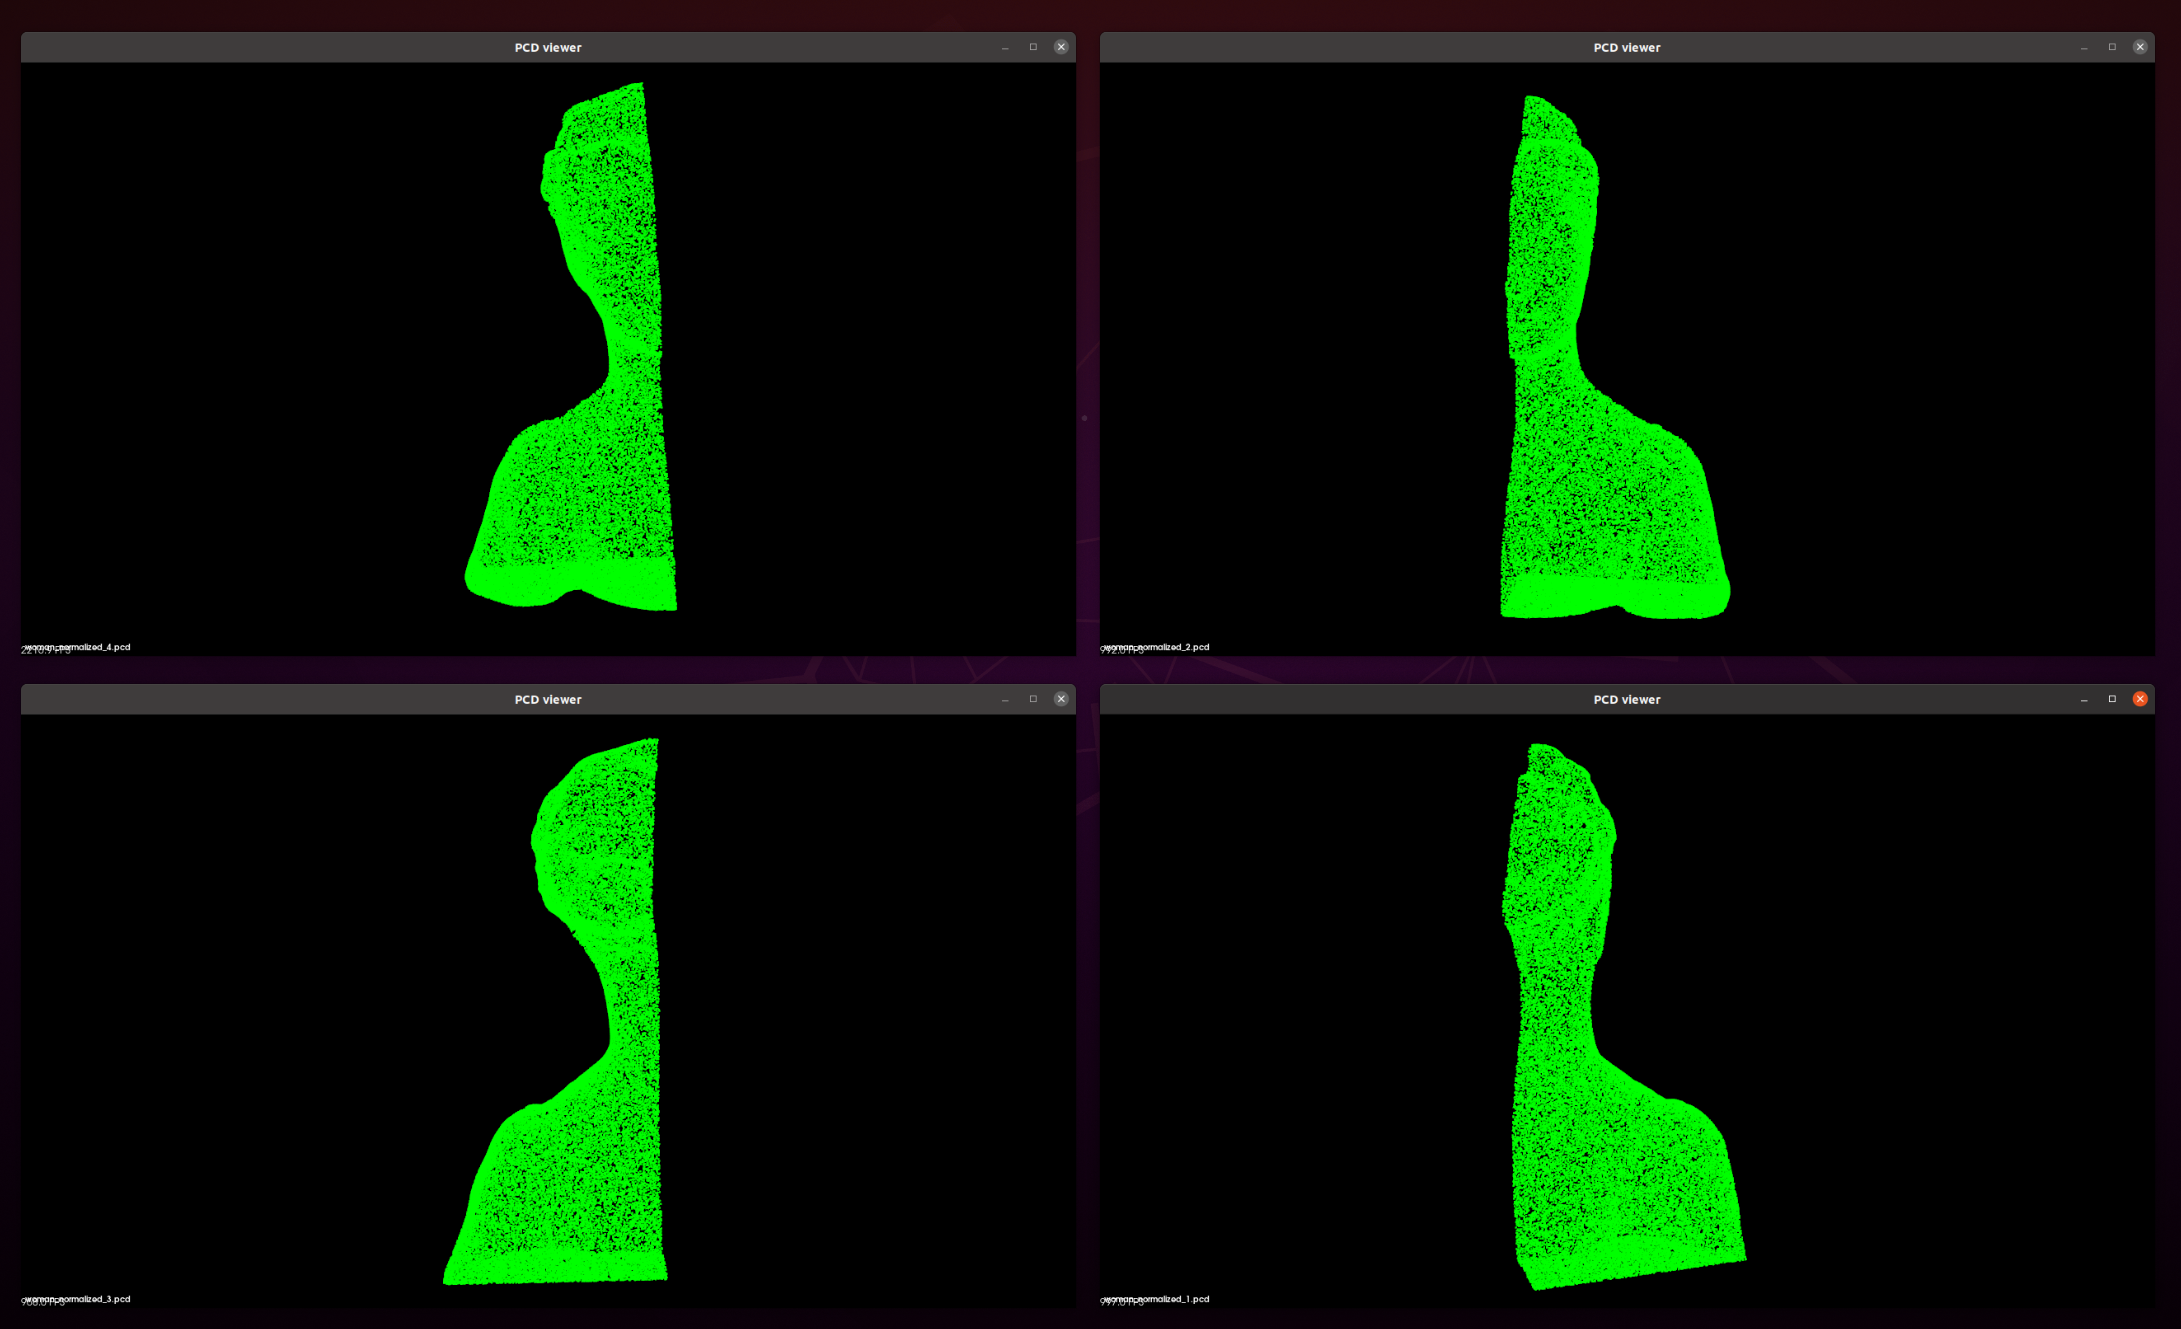
\includegraphics[width=0.5\linewidth]{images/2.png}}
  \caption{Распределение сегментов облака точек по процессам}
\end{figure}


\section{Результаты экспериментов}

Рассмотрим теперь вопрос об эффективности алгоритма. Для этого напомним, что
каждый параллельный алгоритм оценивается по двум параметрам – ускорению $S_p$ и
эффективности $E_p$ , которые определяются по формулам:
$$S_p = {{t_1} \over {t_p}},$$ $$E_p = {S_p \over p} * 100\%$$
где $t_1$ - время решения исходной задачи на одном процессоре, $t_p$ - время
решения исходной задачи по параллельному алгоритму на p процессорах.

Спецификация системы \\
11th Gen Intel® Core™ i7-11800H @ 2.30GHz × 16  \\ 
Число вычислительных ядер: 8


\begin{figure}[h]
    \centering
    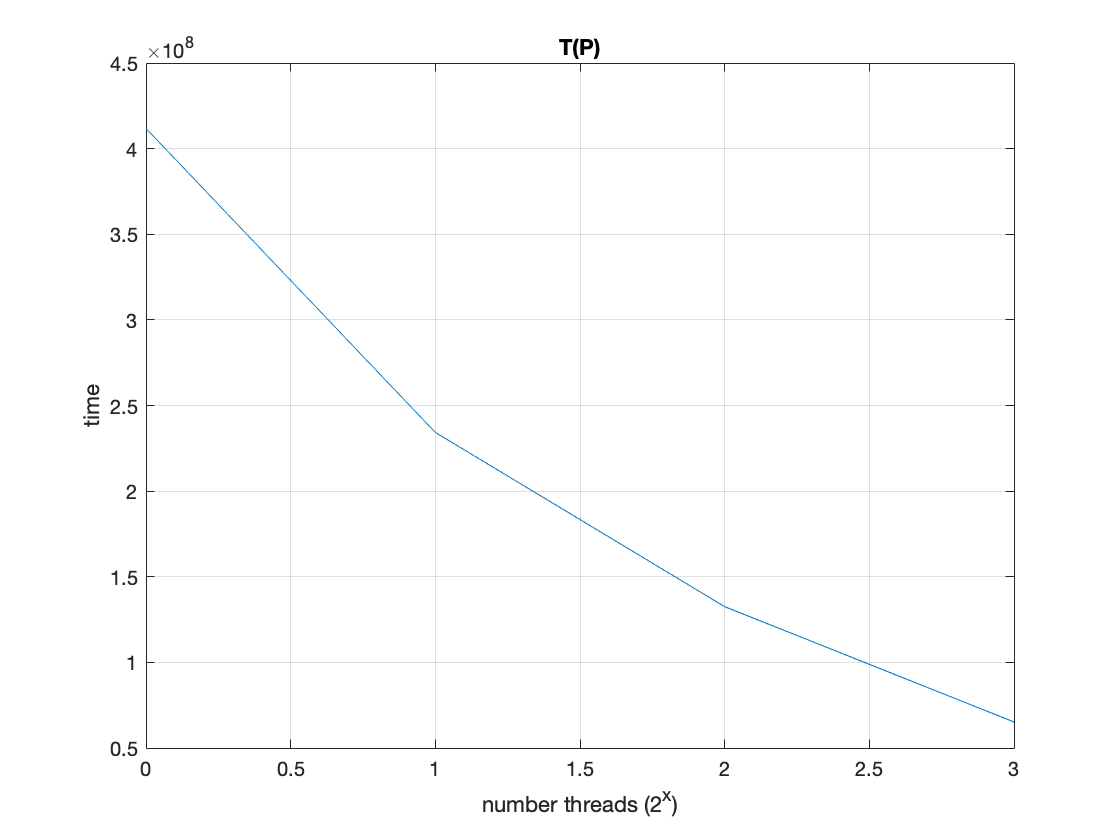
\includegraphics[scale=0.4]{T(P).png}
    \caption{Время работы ($\mathbf{ns}$) на n процессах n = 1...8}
    \label{fig:mesh1}
\end{figure}

\begin{figure}[h]
    \centering
    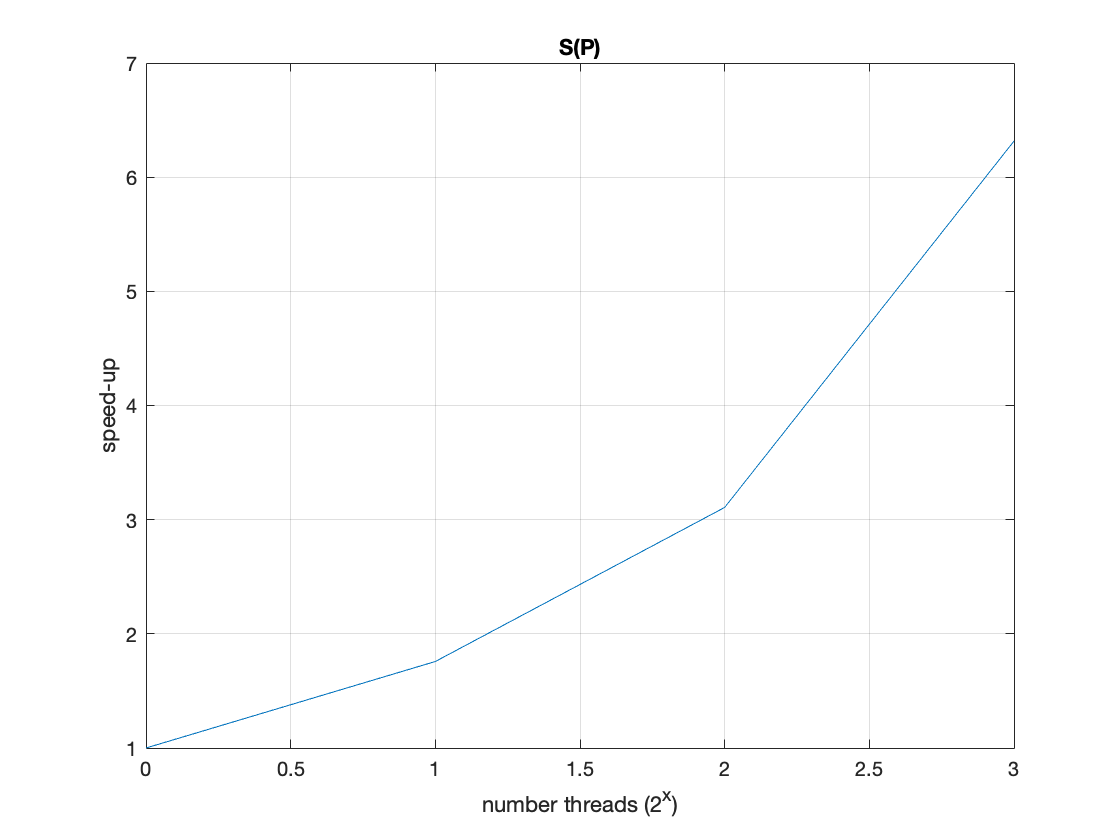
\includegraphics[scale=0.4]{S(P).png}
    \caption{Ускорение}
    \label{fig:mesh1}
\end{figure}

\begin{figure}[h]
    \centering
    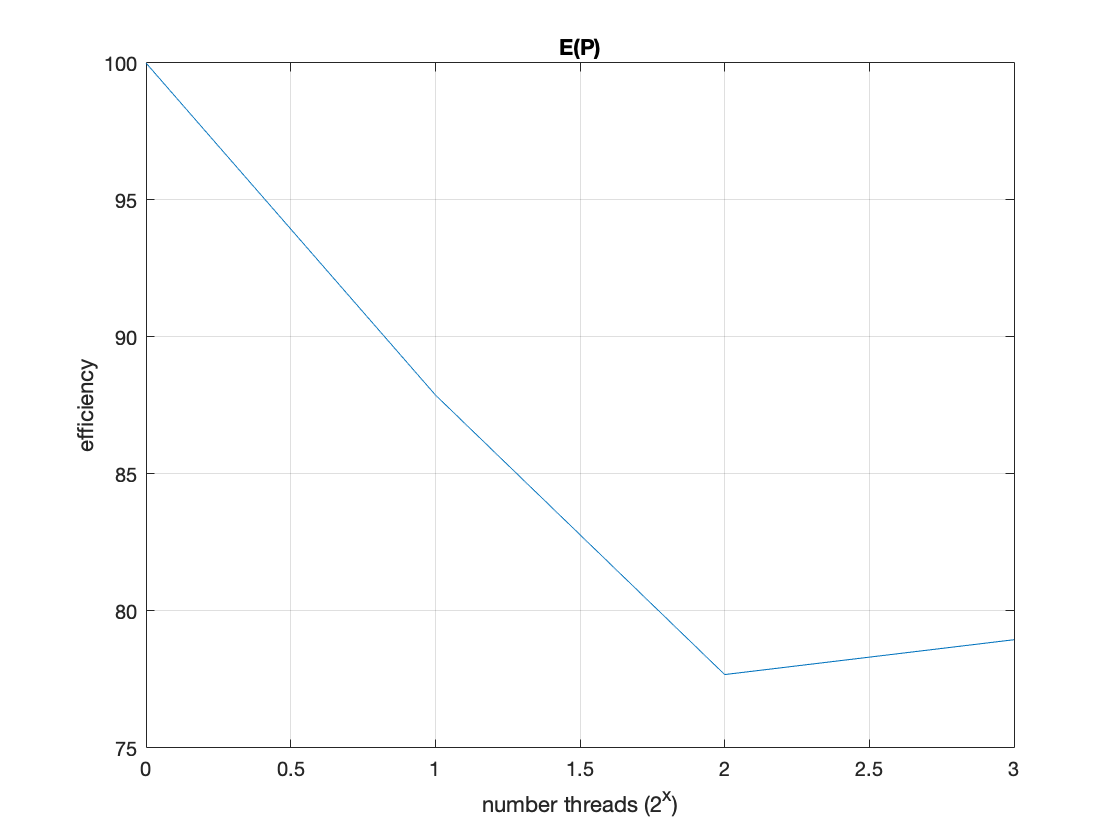
\includegraphics[scale=0.4]{E(P).png}
    \caption{Эффективность}
    \label{fig:mesh1}
\end{figure}




